%# -*- coding: utf-8-unix -*-
%%==================================================

\chapter{开放数据集的学习}

\section{Towards Open World Object Detection}

参考\href{https://zhuanlan.zhihu.com/p/357143607}{目标检测一卷到底之后,终于又有人给它挖了个新坑|CVPR2021 Oral}

通常情况下,对于一个未知的事物,第一次碰到它我们首先会在脑海里做个标记,接着我们会怀着好奇心去学习相关知识,去了解这个未知的事物。如果第一次没有做标记,不去补充相应知识的话,下次再碰到它,我们还是不认识。对于开放世界的目标检测,作者将上面这种增量学习的思想用在开放数据集上模型的学习(对于开放数据集的相关知识,可以参考最后一小节),取得了很好的效果。

\subsection{问题的提出}

作者指出了闭集学习在开放世界检测中存在的问题:
\begin{itemize}
    \item COCO,VOC数据集的类别在开放世界中是相当少的,因此将未知的事物归纳为未知的应具有很好的泛化能力。
    \item 在公开数据集上取得的图像分类的进步,不能轻易地适应“开放世界”的物体检测,主要原因是检测器将unkown的物体检测为背景(负样本)。
    \item 即使是在公开数据集上取得很好性能的模型也会出现假阳性(FP)的检测,比如会将unkown物体检测为某一个known类,而且概率还很高。
    \item 世界是多元和动态的,对于某一个类别,在数目,样式和比例上理应是不同的,因此开发世界的物体检测比封闭世界通过静态学习更加自然,对于目标检测的实践部署,比如机器人,自动驾驶,医疗护理,监视程序并不能完全学习所有的类别。
\end{itemize}

本文的研究方向:Open Set learning + few shot learning,如图\href{fig:2-1}{2-1} 所示。

\begin{figure}
  \centering
  % Requires \usepackage{graphicx}
  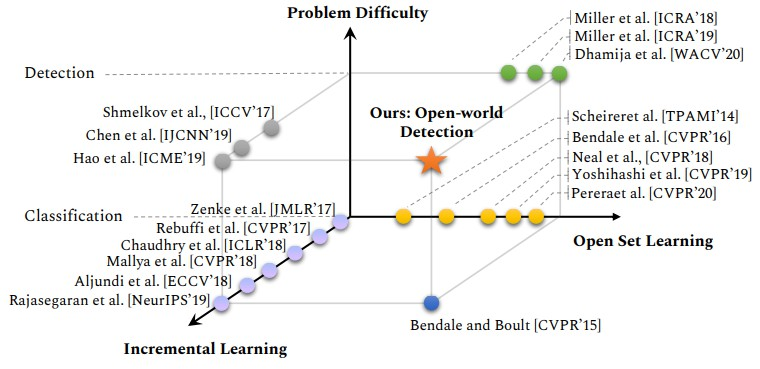
\includegraphics[width=4.5in]{figure/example/OpenSet6.jpg}
  \caption{作者研究的方向}
  \label{fig:2-1}
\end{figure}

本文创新点是:
\begin{enumerate}
    \item 在没有明确监督的情况下,将未被引入的物体识别为“未知”
    \item 当接收到相应的标签时,在不忘记之前学过的类的情况下,逐步学习之前识别出的未知类别。
    \item 该方法在增量目标检测中取得state of art 的性能。\\
\end{enumerate}

要想进行“开放世界的目标检测“,首先需要给出相应的定义:在任何时间$t$,我们都将已知的目标类别集合视为 $K^t = \{1,2,...,C\} \subset \mathds{N}^+$ ,其中$\mathds{N}^+$表示正整数集合。

为了更真实的模拟现实世界,作者假设存在一组未知类别$U = \{C+1,...\}$。

假定已知目标类别$\kappa_t$在数据集$D^t = \{X^t,Y^t\}$中被标记,其中$X^t$和$Y^t$分别表示输入图像和标签。

输入图像集包括$M$个训练图像$X^t = \{I_1,...,I_M\}$,每个图像的相关对象标签形成标签集$Y^t = \{Y_1,...,Y_M\}$。

每个$Y_i=\{y_1,y_2,...,y_k\}$编码一组带有其类别标签和位置的$K$个对象实例,即 $y_k=[l_k,x_k,y_k,w_k,h_k], \quad l_k \in \kappa^t$,其中$x_k,y_k,w_k,h_k$分别表示边界框的中心坐标,宽度和高度。

开放世界的目标检测设置考虑了目标检测模型$M_C$,该模型经过训练可以检测所有先前遇到的$C$对象类。重要的是,模型$M_C$能识别属于任意已知$C$类的测试实例,并能通过将其分类为未知类来识别新的或不可见的类别实例。未知的实例集$U^t$将反馈给可以定义$n$个新类别的使用者,并为此提供训练实例。因而逐渐添加$n$个新类别并进行迭代,以生成新模型$M_{C+n}$,实现模型的增量学习。

文章的整体框架图\href{fig:2-1}{2-1}所示。
\begin{figure}
  \centering
  % Requires \usepackage{graphicx}
  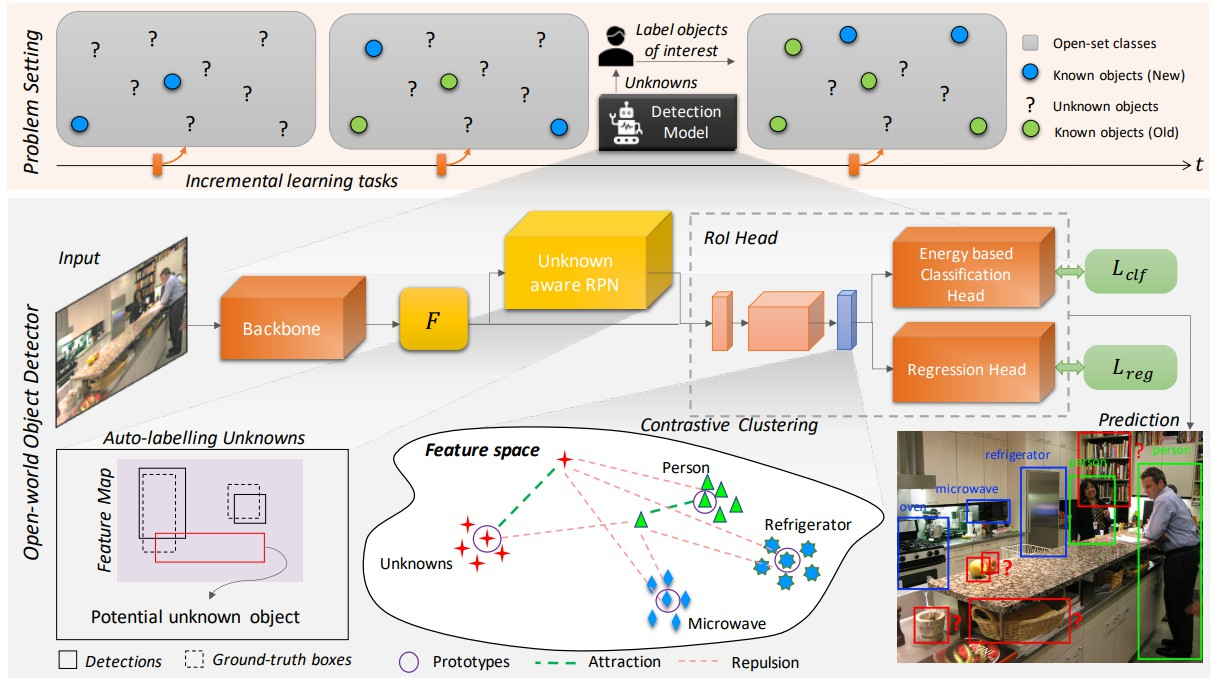
\includegraphics[width=5.5in]{figure/example/OpenSet5.jpg}
  \caption{Open World Object Detector整体框架图}
  \label{fig:2-1}
\end{figure}

\subsection{解决方案}

成功的开放世界目标检测方法应能够在没有明确监督的情况下进行未知实例的识别,并能将识别出的新实例标签提供给模型进行知识升级,同时不会忘记之前的实例,且无需从头开始重新训练。本文提出的ORE便能一并应对这两个挑战。

ORE(Open World Object Detector)在设计上主要包括4个方面:对比聚类(Contrastive Clustering),使用RPN进行未知类别的自动标注,基于未知识别的能量检测(Energy Based Unknown Identifier),失忆性的消除(Alleviating Forgetting)。对于unknown实例的识别,不使用监督学习,而是采用Contrastive Clustering,并利用RPN自动标注机制,将样本划分成0或1,这有助于在潜在空间中利用能量检测划分known和unknown类。

\subsubsection{对比聚类(Contrastive Clustering)}
对于每个已知类$i \in \kappa^t$,保留原型向量$p_i$。令$f_c \in R^d$是由目标检测器中间层对$c$类对象生成的特征向量。我们将对比损失定义如下:
\begin{align}
& L_{cont}(f_c) = \sum_{i=0}^C l(f_c,p_i), where \nonumber \\
& l(f_c,p_i) =
\begin{cases}
D(f_c,p_i) \quad  i = c \\
max\{0,\Delta -D(f_c,p_i)\} \quad otherwise
\end{cases}
\end{align}

当$i = c$时,$p_i$是$c$类的原型(类)向量,此时计算原型向量$p_i$和输入的特征向量$f_c$的类内距离$D(f_c,p_i)$; 否则计算$max\{0,\Delta - D(f_c,p_i)\}$,其中$\Delta$是一个超参数,表示人为拟订的相似和非相似类别之间的距离,如果$D(f_c,p_i) > \Delta$,则两个类别在聚类中可以完全区分开,损失值为0。

通过对上面损失函数的最小化,可以实现潜在空间中不同类别的分离。其中类别原型向量$P = \{p_0,p_1,...,p_c\}$是ORE的重要组成部分,以$p_c$为例,它是输入特征向量$f_c$构所成的队列$q_c$经过求均值之后得到的向量。因此相应的,对于多类别的输入特征向量,可以用$F_{store} = \{q_0,q_1,...,q_c}$ 来存储$c$个类别的特征向量,假设队列$q_i$的固定长度为$Q$,则$F_{store}$是一个$C \times Q$的矩阵。

对比聚类算法图\href{fig:2-1}{2-1}所示。在该算法中,$I_b$是一个超参数,表示迭代的次数,当$i == I_b$时,可以计算初始的原型向量$p_i$(即取$q_i$的mean 值)和$p_i$和$f_c$的损失值;当$i > I_b$时,设置另一个超参数$I_p$,当$i \% p == 0$ 时,得到$p_{new}$(即取$q_i$的mean值),接着更新原始向量:$p_i \leftarrow \eta p_i + (1-\eta)p_{new}$,其中$\eta$表示学习率。
%算法
\begin{figure}
  \centering
  % Requires \usepackage{graphicx}
  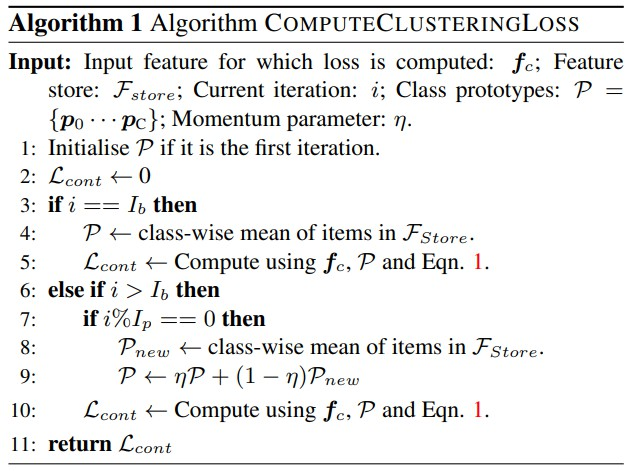
\includegraphics[width=3.5in]{figure/example/openset4.jpg}
  \caption{对比聚类算法}
  \label{fig:2-1}
\end{figure}

\subsubsection{RPN进行unknown类别标注}
在对比聚类之前,我们需要用unknown的真实框来标记unknown的对象实例,而在已标注的大规模数据集中重新标注每个图像的所有实例显然是不切实际的。作为替代,作者建议自动将图像中的一些对象标记为潜在的unknown 对象。在实验中,作者发现Faster R-CNN在开放数据集上的学习比Yolo,retinaNet好,为此,作者采用RPN(区域建议网络)将那些具有较高置信度(confidence) 但不与ground-truth对象重叠的propasal标记为潜在的未知对象。本文中RPN的使用和Faster R-CNN中的基本相同,这里补充一下Faster R-CNN中RPN相关知识:

在Faster R-CNN中,RPN利用多尺度的锚框替代了耗时的Selected Search算法进行正负候选区域的提取。RPN共有两层,第一层为cls层(即框分类层),会给该框打分,得分由两个部分组成:一是该物体的分类概率,二是判断该框中对象是否为物体;第二层为reg层(即框回归层),会给该框标注坐标,坐标包括四个部分:锚框的中心坐标(x,y),锚框的宽高(w,h)。Faster R-CNN网络结构如图
\href{fig:2-2}{2-2}所示。

\begin{figure}
  \centering
  % Requires \usepackage{graphicx}
  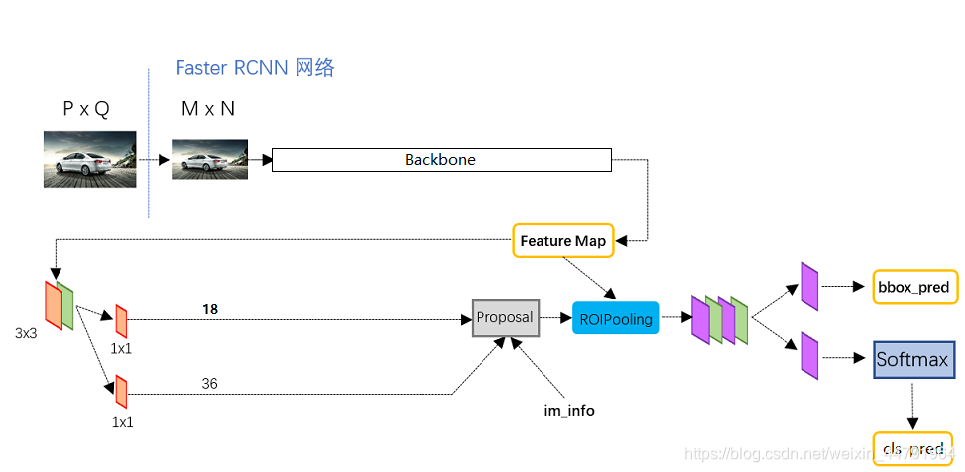
\includegraphics[width=4.5in]{figure/example/faster_RCNN.png}
  \caption{Faster R-CNN网络结构图}
  \label{fig:2-2}
\end{figure}

\subsubsection{基于未知识别的能量检测(Energy Based Unknown Identifier)}

给定潜在空间$F$中的特征$(f \in F)$及其对应的标签$l \in L$,我们使用基于能量的模型(EBMs)来学习一个能量函数 $E(F,L)$。对于落在分布内的数据$(f,l)$,通过EBMs建模,我们会得到一个低能量值,这个值表示$(f,l)$匹配稳定,反之亦然,这使得我们可以通过能量度量来表征样本是否来自未知类别(能量模型相关知识请见最后一小节)。这里作者使用亥姆霍兹自由能公式将$L$中所有类别的能量组合在一起,得到$E(f)$,亥姆霍兹自由能方程如下:
\begin{align}
&E(f) = -Tlog\int_{l'}exp(-\frac{E(f,l')}{T})
\end{align}

其中$T$是温度参数。使用softmax函数来计算$label = l$在输入特征向量$f$下的概率密度$p(l|f)$,最简单能量建模方法就是利用$f,l$的吉布斯(Gibbs)分布来描述$f,l$之间的能量,因此softmax中的值是每个类别特殊能量值的吉布斯分布$g_i(f)$,$p(l|f)$计算公式如下:
\begin{align}
& p(l|f) = \frac{exp(\frac{g_l(f)}{T})}{\sum_{i=1}^C exp(\frac{g_i(f)}{T})} = \frac{exp(-\frac{E(f,l')}{T})}{exp(-\frac{E(f)}{T})}
\end{align}

其中$g_l(f) = -E(f,l)$,将$\sum$挪到$exp()$里面,关于全类别的条件期望 $=$ 无条件期望。

结合上面两个式子,作者将分类模型的自由能定义如下:
\begin{align}
E(f;g) = -Tlog \sum_{i=1}^C exp(\frac{g_i(f)}{T})
\end{align}

该函数装在Faster R-CNN的头部,作者先通过Contrastive Clustering对不同类别进行划分(包括unknown对应的0类),再利用该能量函数观察每个类别的energy水平。在探索性分析中,作者比较了Gamma,Exponential,Normal,Weibull分布,发现用Weibull分布来描述图\href{fig:2-3}{2-3}中known和unknown 类别的真实分布更加合适。从图\href{fig:2-3}{2-3}可以发现,known类别的能量小于unknown类别的能量($\varepsilon_{kn}(f) < \varepsilon_{unk}(f)$)

\begin{figure}
  \centering
  % Requires \usepackage{graphicx}
  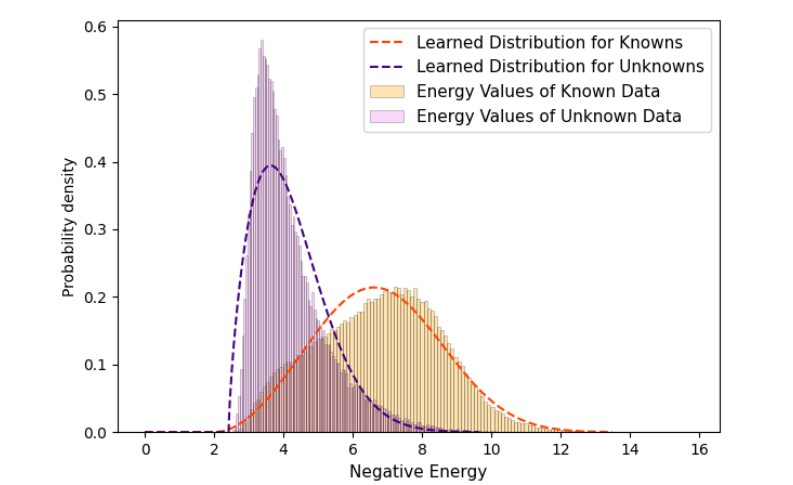
\includegraphics[width=5in]{figure/example/openset3.jpg}
  \caption{known和unknown类别的能量分布}
  \label{fig:2-3}
\end{figure}

\subsubsection{失忆性消除(Alleviating Forgetting)}

在失忆性消除(保留记忆性)中,模型不会再进行学习之前Train数据集中的数据,因为如果从头开始训练unknown 类别的话不仅会相当耗时,而且如果只是学习新类别的话,会忘记之前学习的类,无法实现增量学习。这里作者列举了几个记忆性保留的方法:参数标准化,样例重播,动态延伸网络和元学习。Prabhu\cite{prabhu2020gdumb} 采用贪心选择策略进行样例的重播, Wang\cite{wang2020frustratingly}在few shot detection中,提出了通过存储少量样例来进行样例重播的方法。作者在本文中采用后者提出的方法,先是存储平衡的unknown样例集,并在每一步增量学习中进行模型的精调(finetune),保证每个类别的样例个数最小化的N个(就好比在为自己的算法设计测试用例时,同个if内的样例是等价的,只需保留一个即可)。

简单来说,就是使用已经通过大量数据集训练好的base模型,并在该模型的后面增加一些层进行少样本的训练,对模型进行精调(few shot learning),这里的base模型好比预训练模型。相关知识请参考本章最后一小节。

\subsubsection{细节问题:一些超参数的设置}

1、margin($\Delta$)的设置如图\href{fig:2-4}{2-4} 所示。作者发现增大$\Delta$值可以提高已知类和未知类的区分性能,即有利于在潜在空间中ORE对known,unknown类进行分离。

\begin{figure}
  \centering
  % Requires \usepackage{graphicx}
  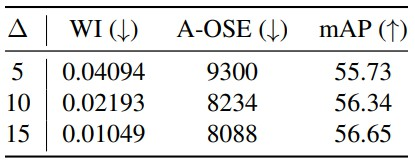
\includegraphics[width=2.5in]{figure/example/ORE2.jpg}\\
  \caption{margin($\Delta$)的设置}
  \label{fig:2-4}
\end{figure}

2、$F_{store}$中队列长度$Q$的设置如图\href{fig:2-5}{2-5}所示。作者发现,改变原型向量$p_i$的计算数量不会对性能产生巨大影响。
\begin{figure}
  \centering
  % Requires \usepackage{graphicx}
  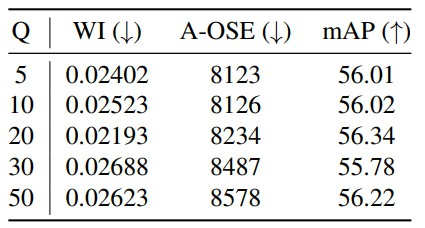
\includegraphics[width=2.5in]{figure/example/ORE1.jpg}\\
  \caption{$F_{store}$中队列长度$Q$的设置}
  \label{fig:2-5}
\end{figure}

3、亥姆霍兹自由能方程中温度$T$的设置如图\href{fig:2-6}{2-6}所示。作者发现,温度参数在$T = 1$和$T = 2$之间存在一个很好的平衡点,可以提供最佳性能。
\begin{figure}
  \centering
  % Requires \usepackage{graphicx}
  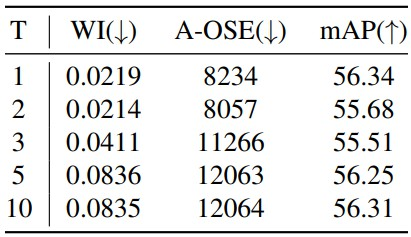
\includegraphics[width=2.5in]{figure/example/ORE3.jpg}\\
  \caption{亥姆霍兹自由能方程中温度$T$的设置}
  \label{fig:2-6}
\end{figure}

4、对比聚类算法中学习率$\eta$的设置如图\href{fig:2-7}{2-7}所示。作者发现,$\eta$值越大,ORE分离unknown,known类的性能越好,这意味着类原型的逐步发展会改善对比聚类。
\begin{figure}
  \centering
  % Requires \usepackage{graphicx}
  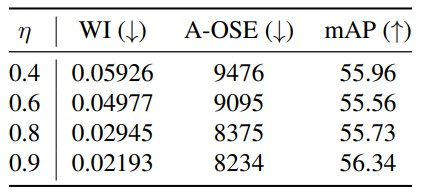
\includegraphics[width=2.5in]{figure/example/ORE4.jpg}\\
  \caption{对比聚类算法中学习率$\eta$的设置}
  \label{fig:2-7}
\end{figure}

\subsection{实验结果}

在图\href{fig:2-10}{2-10}中,作者使用Pascal VOC数据集训练base模型(如Task1),接着将MS-COCO数据集划分成3个,进行增强学习(如Task2,Task3,Task4)。在实验中,作者定义了两种度量指标:开放影响WI和开放数据集绝对误差A-OSE:
\begin{align}
&Wilderness Impact(WI) = \frac{P_K}{P_{K \cup U} - 1 
\end{align}
其中$P_K$是模型在使用known类别数据集进行训练时Known类别的precision,$P_{K \cup U}$是模型在使用Known,Unknown类别进行训练时Known,Unknown类别的precision。WI越小,表明unknown类别的加入不会很大影响原来的known类别的检测精度。

\begin{figure}
  \centering
  % Requires \usepackage{graphicx}
  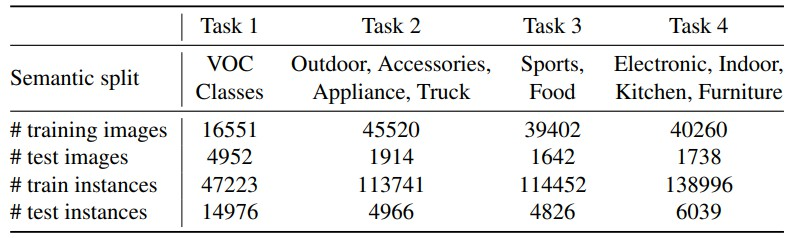
\includegraphics[width=5in]{figure/example/ORE5.jpg}\\
  \caption{实验任务实施计划}\label{}
\end{figure}

在图\href{fig:2-11}{2-11}中,作者使用4个模型进行对比分析:一个是"Oracle"检测器,它是在ORE模型的基础上对所有的known,unknown带标签的类别进行训练,是最理想的训练方式,目的是为了和性能优越的ORE模型进行比较;另一个是使用ResNet-50 的Faster R-CNN;再一个是在Faster R-CNN基础上使用增量学习的模型,最后一个是ORE模型。通过图\href{fig:2-11}{2-11},我们可以看到Faster R-CNN 在学习新的类别时会忘记之前已学习的类别,ORE和Faster R-CNN却不会存在这个问题。而相比于ORE和Faster R-CNN + finetune,ORE在WI,A-OSE指标上性能更加优越,并且和理想状态下的"Oracle"差距不是很大。

\begin{figure}
  \centering
  % Requires \usepackage{graphicx}
  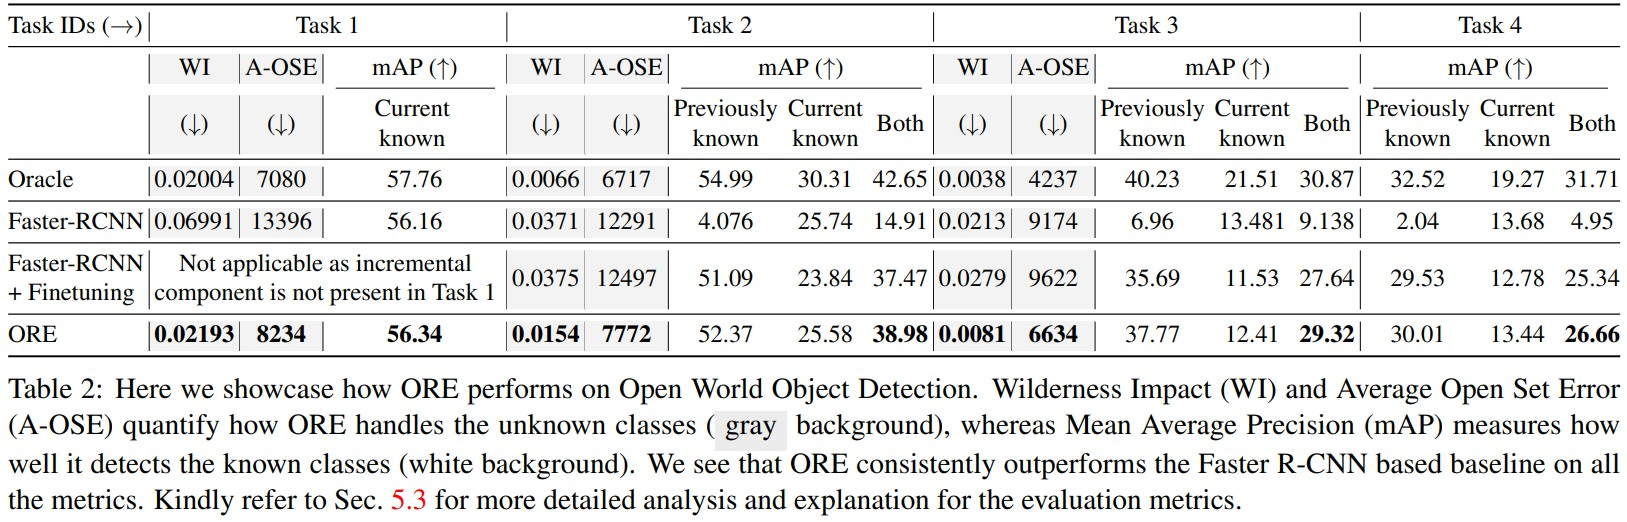
\includegraphics[width=6in]{figure/example/ORE6.jpg}\\
  \caption{ORE和"Oracle",Faster R-CNN,Faster R-CNN + finetuning的比较}
  \label{}
\end{figure}

由图\href{fig:2-11}{2-11}所知,ORE已经完胜了Faster R-CNN,接着作者着重分析了ORE和增量式目标检测器在性能上的区别,如图\href{fig:2-12}{2-12}所示。通过3种不同的设置,ORE和最新的增量式目标检测器ILOD进行比较,发现ORE 在所有设置中都表现十分出色。
\begin{figure}
  \centering
  % Requires \usepackage{graphicx}
  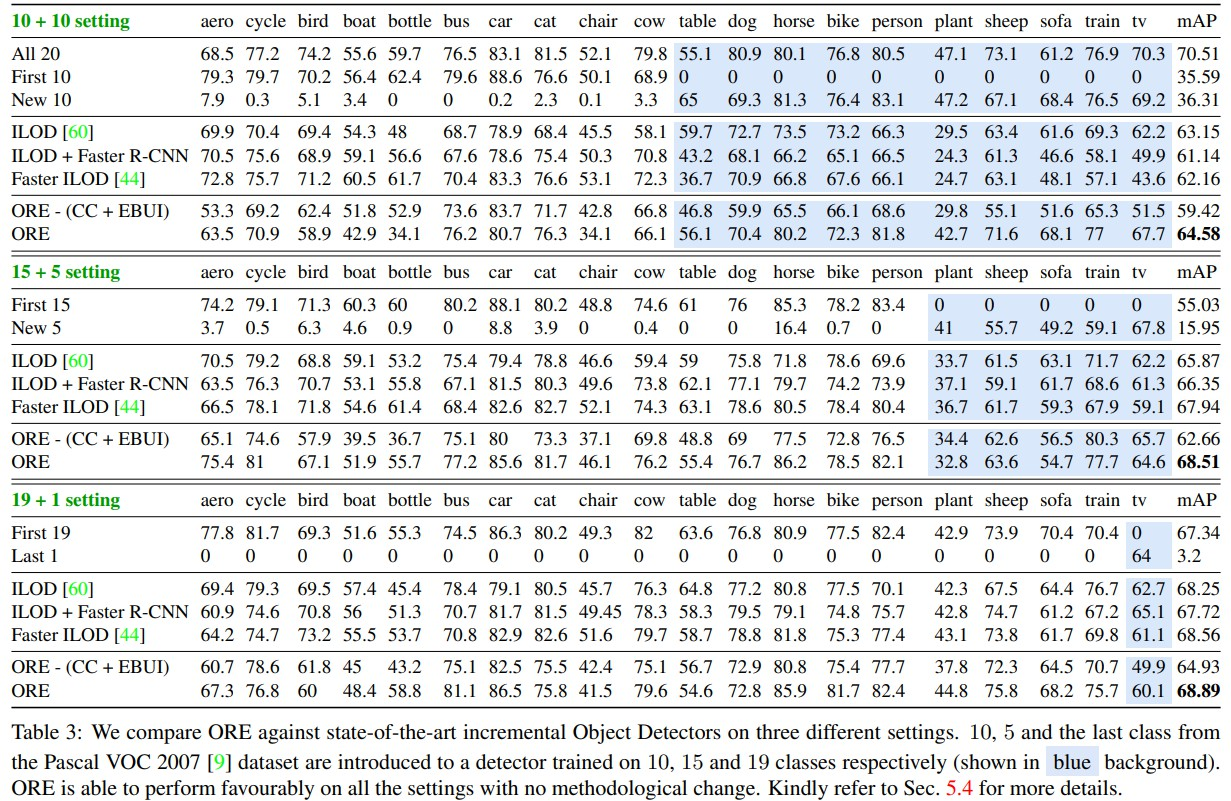
\includegraphics[width=6in]{figure/example/ORE7.jpg}\\
  \caption{ORE和增量检测器的比较}
  \label{}
\end{figure}

少样本样例数$N_{ex}$设置如图\href{fig:2-13}{2-13}所示。
\begin{figure}
  \centering
  % Requires \usepackage{graphicx}
  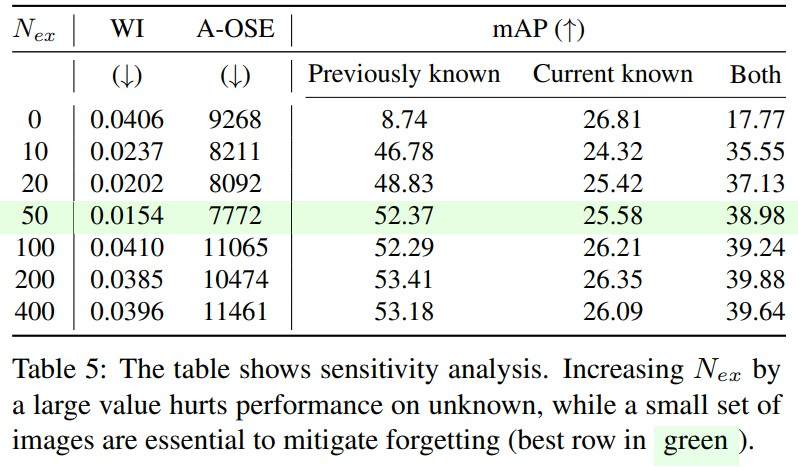
\includegraphics[width=4.5in]{figure/example/ORE9.jpg}\\
  \caption{少样本样例数$N_{ex}$设置}
  \label{}
\end{figure}

Contrastive Clusting的聚类结果如图\href{fig:2-14}{2-14}所示。
\begin{figure}
  \centering
  % Requires \usepackage{graphicx}
  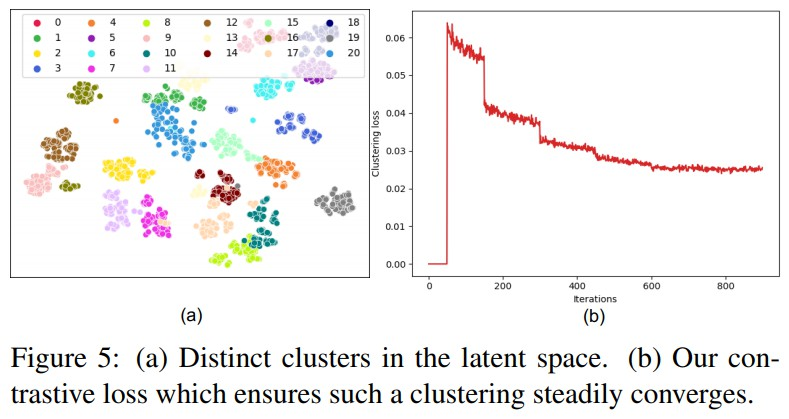
\includegraphics[width=5in]{figure/example/ORE8.jpg}\\
  \caption{Contrastive Clusting的聚类结果}
  \label{}
\end{figure}


\subsection{小总结}

本文作者认为,基于有限类别的数据集进行的模型训练,得到的模型不利于对开放世界数据集的检测,即使在公开数据集上性能表现很好的模型,在真实世界上也会出现假阳性检测问题,而且置信度还很高。因此作者本文的研究方向是:Open set learning + few shot learning(不包含incremental learning,因为其不需要对前面训练结果进行存储,而ORE需要对少量的unknown数据集进行存储),目的是利用模型在公开数据集上检测出来的unknown类别,进行少样本的incremental learning,对模型进行精调。

在实现上,作者先是通过Faster R-CNN的RPN网络筛选出正负样本,其中的负样本就是unknown类别;接着对所有类别进行无监督的Contrastive clustering,使不同类别落在各自的角落(unknown类别为0 类);接着使用能量模型,对known和unknown类别进行能量检测,由于之前已经使用过对比聚类,能量检测也会更加容易。能量检测的理想结果是known类别的能量小于unknown类别的能量,也就是known类别比unknown类别稳定;接着通过探索性分析,得出known和unknown类别在能量上近似于WeillBull分布。最后存储之前具有代表性(分布)的少量unknown样例(应该需要人工添加类别标签),进行少样本的学习(few shot learning),这里的少样本个数由一个超参数来设置$N_{ex}$。\\

谈谈我的感悟:我之前貌似也有类似零零散散的点子,如果把这篇论文的点子比作是一片大海,我的点子就是那海边的小沙子。看到有人实现了这个点子,很开心,毕竟解决了我一个困惑。之前我使用Faster R-CNN 训练自己标注的,具有两个标签的数据集(数据集不大,只有30 张easy$\_$hand,50张mid$\_$hand,25张easy$\_$wheel,45张mid$\_$wheel)。一开始我只是标注了easy$\_$hand(手部没有遮挡)并进行模型的训练,发现模型过拟合,原因可能是在采集的图片中手部姿势过于单一,大多存在重复。因此我就有了第一个想法:能否在图片训练过程中,有个预处理过程,用来判断不同图片的ground truth (真实框)中hand的相似度,保留具有代表性的图片类别样例,避免相似图片重复训练,导致模型在训练时存在过拟合问题。而在本文中,作者提出了用contrastive clustering进行类别的对比聚类,输入数据包括输入的特征向量$f_c$ 和类别$l$,虽然这种方法不能解决相似类别图片重复性训练问题,但是却能清楚的看到该类别下深度提取的特征的散落位置,可以分析特征之间的相似程度。因此第一个想法不太可行,因为预处理的特征比较浅,判断相似度不太靠谱。

接着我再标注mid$\_$hand(有简单的遮挡)并进行模型的训练,发现检测效果一般,会把正脸中的耳朵错检为hand,接着我就在数据集中增加了一些正脸的图片,发现耳朵被检测成hand的几率有所减少,但还是存在,这说明hand和ear在深度提取的特征上存在相似性,才会导致误检。我暂时能想到的解决方法是增加数据样本,使得两者在深度提取的特征中能更好地区分开。对于这个问题,作者在这篇文章中没有提出解决方法,因为文章中识别的known和unkown类别在深度提取的特征(即在潜在空间)中,是存在一定的区别的,就好比现在机器学会如何检测人脸,接下来对于人脸类别相差较大的冰箱(unknown) 类别来说,通过之前训练时存储的少量样本进行学习,就能很好地检测其他数据集中的冰箱类别,模型具有很好地泛化能力。但是对于人脸相差较小的hand来说,作者应该没有将其作为少量样本进行训练,而是在base模型(预训练模型)中,通过大量的训练数据提取更加丰富的深度特征,进而解决相似度较小的类别检测问题。

\subsection{补充知识}

\subsubsection{真实世界中的开集识别问题}

1、闭集与开集分类问题

闭集分类问题(closed-set problem),即测试和训练的每个类别都有具体的标签,不包含未知的类别(unknown category or unseen category); 如著名的MNIST和ImageNet数据集,里面包含的每个类别为确定的。以MNIST(字符分类)为例,里面包含了0 $\sim$ 9的数字类别,测试时也是0 $\sim$ 9的类别,并不包含如字母A $\sim$ Z等的未知类别,闭集分类问题即:区分这10个类别\footnote{真实世界中的开集识别问题 \quad \url{https://blog.csdn.net/u010165147/article/details/97490500}}。

开集分类问题(open-set problem)不仅仅包含0 $\sim$ 9 的数字类别,还包含其他如A $\sim$ Z 等等的未知类别,但是这些未知的类别并没有标签,分类器无法知道这些未知类别里面图像的具体类别,如:是否是A,这些许许多多的不同类别图像共同构成了一个类别:未知类别,在检测里面我们叫做背景类别(background),而开集分类问题即:区分这10个类别且拒绝其他未知类别,如图\href{fig:2-1}{2-1} 所示。

简单来说,就是开集中物体的类别比闭集中多了一个unkown类,该类有边界框,但没有真实标签;而在闭集中,这些unkown类没有被label出来。
\begin{figure}
  \centering
  % Requires \usepackage{graphicx}
  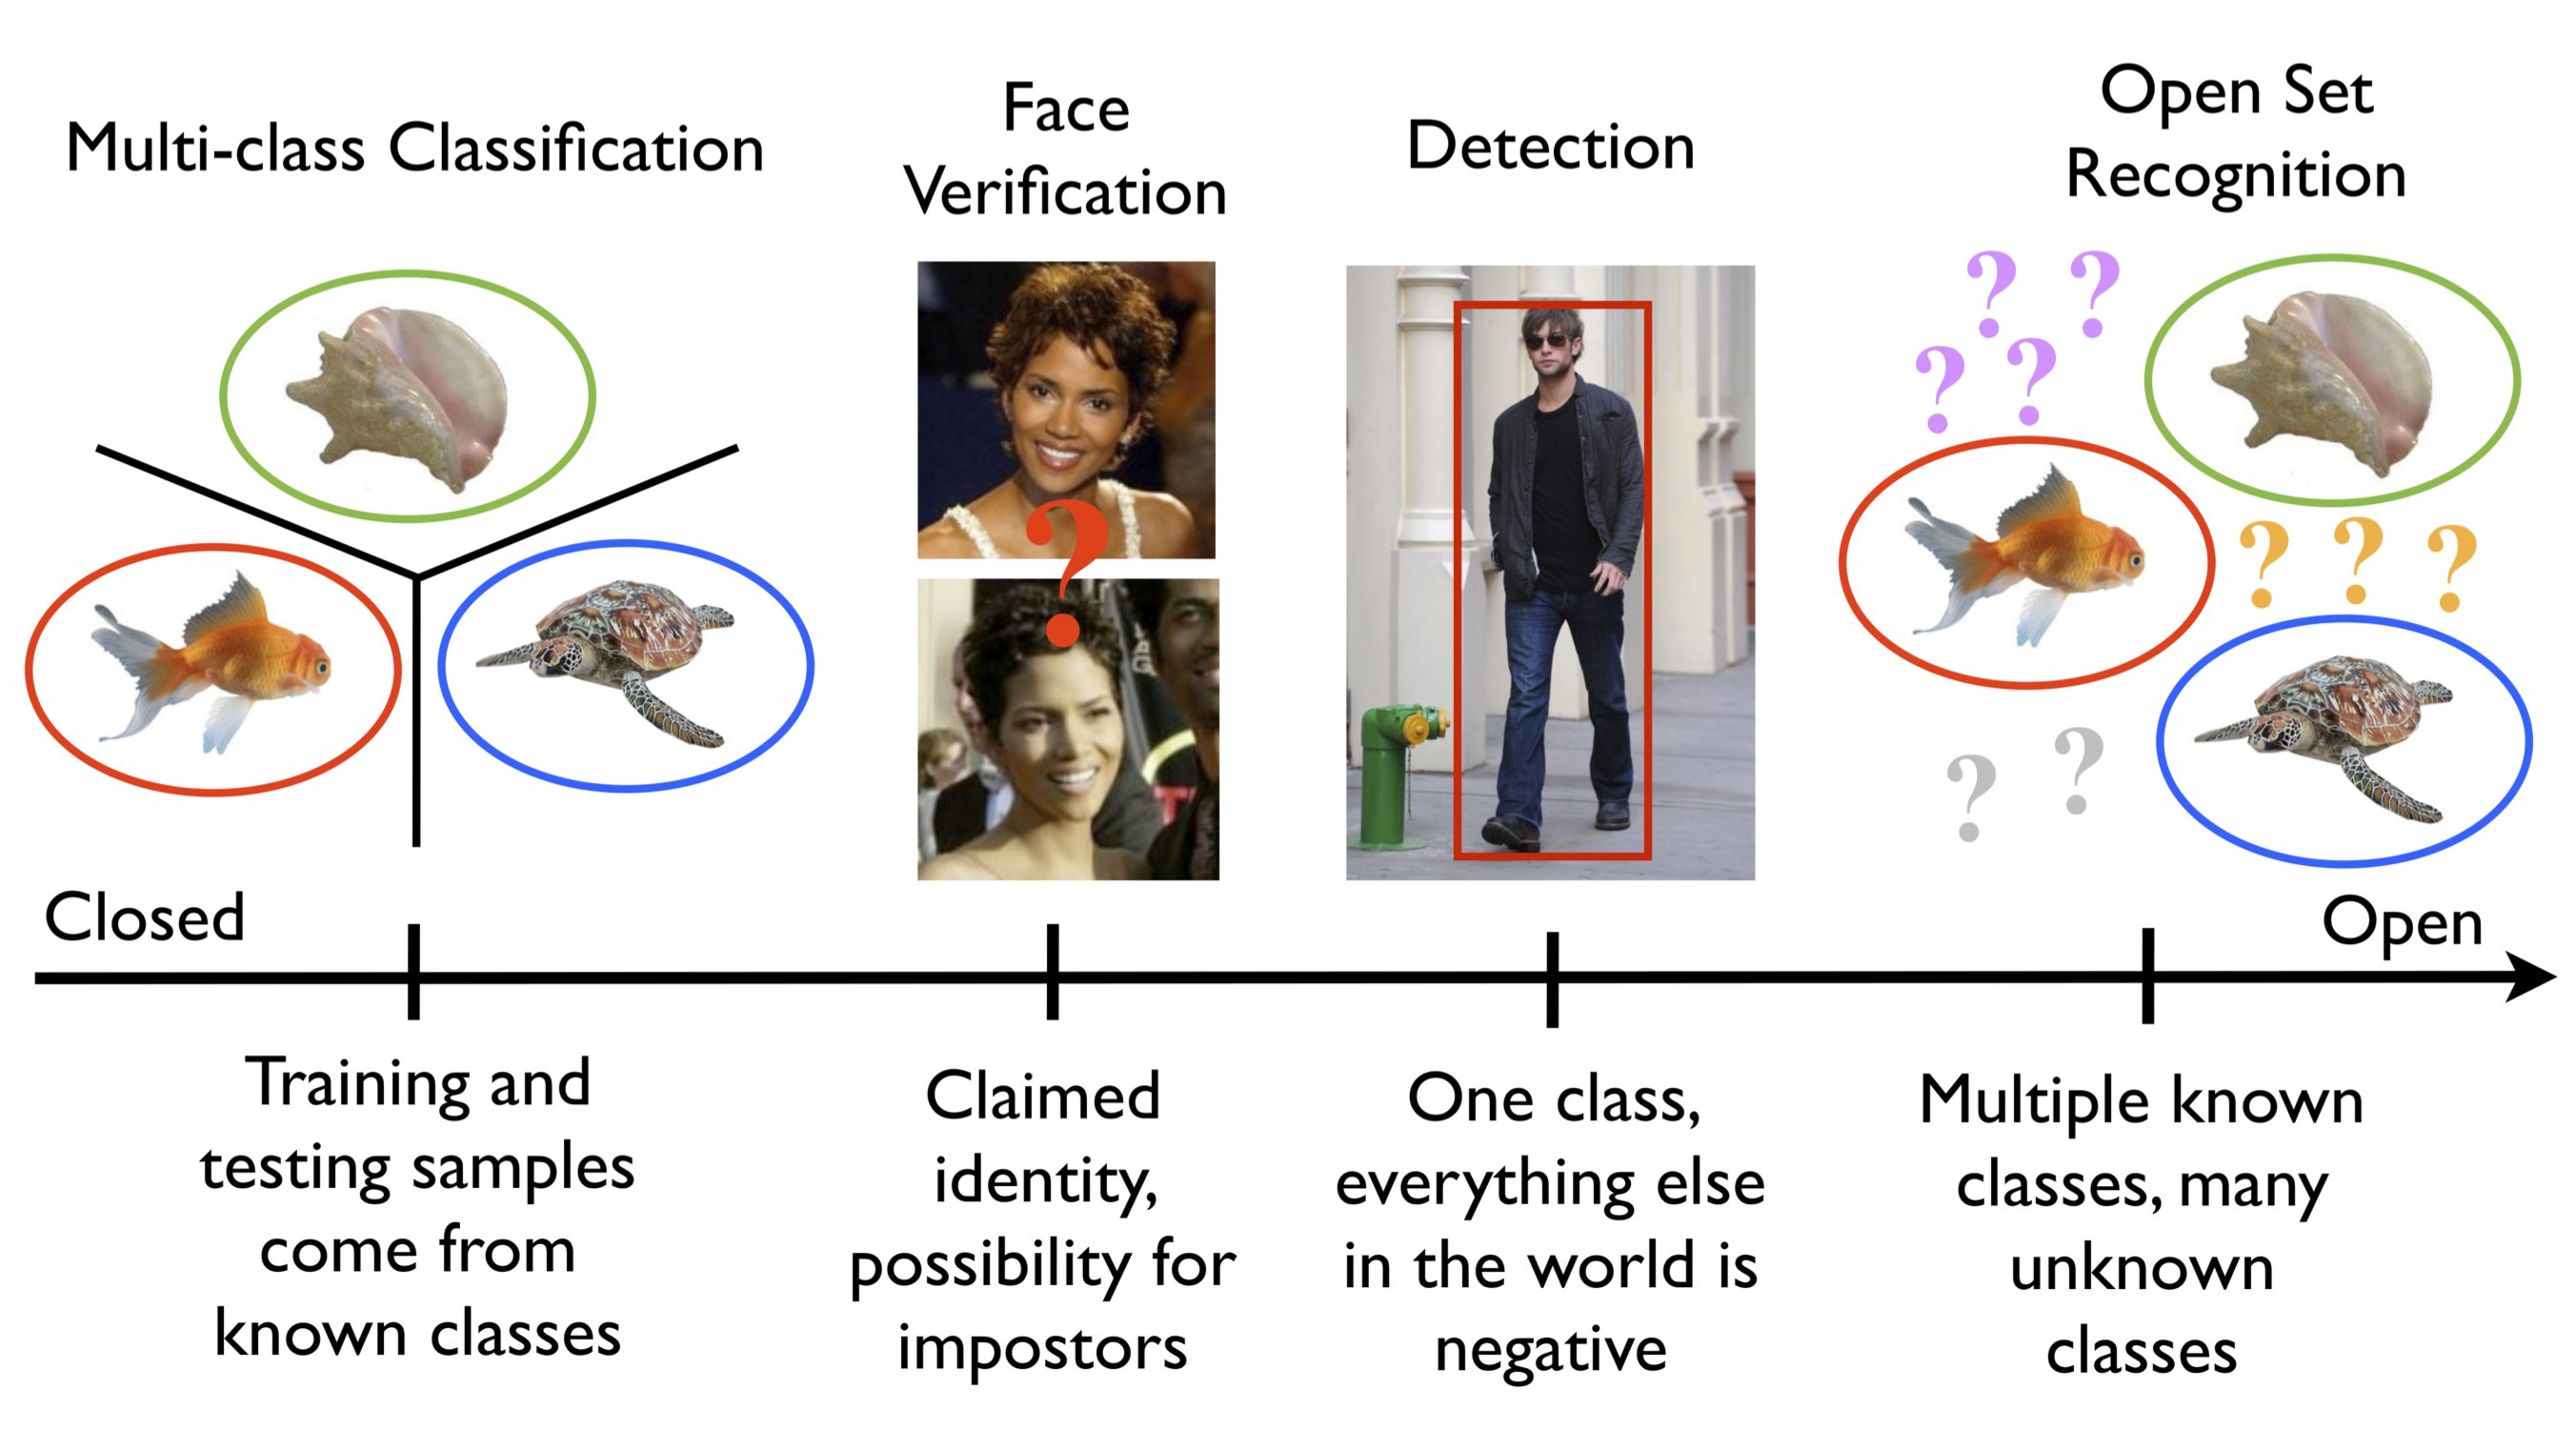
\includegraphics[width=4.5in]{figure/example/OpenSet1.jpg}
  \caption{开集的分类问题}\label{fig:2-1}
\end{figure}

更形式化,可定义为
\begin{itemize}
    \item 闭集分类问题:集合S包含N个有限类别,且该N个类别有具体标签,闭集分类问题即划分这N个类别
    \item 开集分类问题:集合S包含N个有具体标签的有限类别,且S包含K个有限或无限未知类别,开集分类问题即划分这N个类别且拒绝这K个未知类别 \\
\end{itemize}

2、人脸的开集识别问题

通常我们使用的人脸识别技术本身就是open-set problem,即人脸识别的训练集和测试集可能是非常不同的,而闭集测试对于普通的人脸识别商用意义有限,这里就存在测试集的Identities(ID)远远超过训练集的问题; 以微软的开放数据集MS-Celeb-1M为例,它仅仅包含约100K的ID数量,和中国人的ID数相比差了4 个数量级; 那么这个数据集这么小是否就没用的呢?并不是,但是从目前来看ID数量已经成为限制人脸识别精度的主要影响因素,也就是说数据集主要影响的是精度从而影响商用范围(不同的应用要求精度有差别,如社区门禁模型要求在$10^-4$FPR下99$\%$的 TPR 应该说就足够了)

从人脸识别的pipline来看(检测-对齐-识别),人脸识别有两个地方会涉及到open-set问题,第一个就是人脸检测,人脸检测直接面对的就是开放世界的场景,各种各样的物体; 第二个即识别,识别面对的物体要比检测单一,即各种不同ID的人脸。

如果没有检测这一步,人脸识别将会更加困难,这个时候人脸特征失效会非常严重,你无法想象,放一张猫脸或者其他乱七八糟的图片会发生什么。从人脸识别的整个pipline来看,是先拒绝了非人脸,然后再拒绝非注册ID (即级联分类),本质还是拒绝非注册ID,并区分注册ID,而非注册的ID本身就是人脸。所以从定义上说,人脸检测和open-set problem是一致的。

\begin{figure}
  \centering
  % Requires \usepackage{graphicx}
  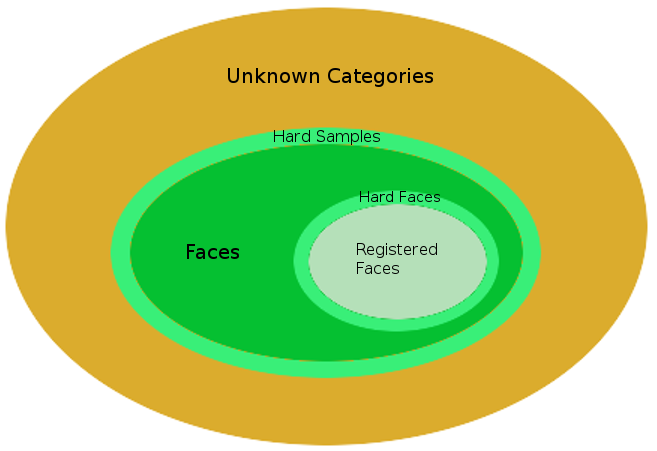
\includegraphics[width=3.5in]{figure/example/openSet3.png}
  \caption{人脸识别的开放集问题}\label{fig:2-3}
\end{figure}

简单来说,当我们在做leetcode算法题时,我们需要事先拟订一些测试用例来检测自己编写的算法是否可行(这里的测试用例好比训练集)。当我们把代码提交上去后,后台会用它自己的测试用例来检验我们的算法(这里的测试用例好比测试集)。如果验证错误,说明我们的训练集和后台提供的测试集有偏差,我们少考虑了某些特殊情况。真实世界下,训练集往往要比测试集小得多。\\

\subsubsection{基于能量的模型(EBMs)和自由能公式}

参考\href{https://www.zhihu.com/question/59264464/answer/203701292}{什么是Energy Based Model(EBM)?},\href{https://github.com/exacity/deeplearningbook-chinese}{deeplearningbook-chinese}

在理解能量模型之前,我们先了解一下无向图模型和无向图模型中的一些基本概念。

有向图模型,比如贝叶斯网络,为我们提供了一种描述结构化概率模型的语言。而另一种常见的语言则是无向图模型(undirected Model),也被称为马尔可夫随机场(Markov randon field,MRF) 或者是马尔可夫网络(Markov network)(Kindermann,1980)。在无向模型中,所有的边都是没有方向的。

当存在很明显的理由画出每一个指向特定方向的箭头时,有向图模型显然最适用,有向图模型可以用来理解具有因果关系以及因果关系有明确方向的情况。而在无向图模型中,两个结点通过
一条边相连接,对应这些结点的随机变量相互之间是直接作用的,但不同于有向图模型的是,这些边是没有方向的,因此并不与一个条件分布相关联,换句话说,并没有明确的条件依赖关系。因此当相互的作用并没有本质性的指向,或者是明确的双向相互作用时,使用无向模型更加合适。

简单来说,有向图模型适合做因果分析,而无向图模型适合做推理分析。\\

一个无向图是一个定义在无向模型$G$上的结构化概率模型。对于图中的每一个团$C$(图中的每个结点之间都有边的连接),一个因子(factor)$\phi(C)$(也称为团势能(clique potential))衡量了团中变量每一种可能的联合状态所对应的密切程度,这些因子是非负的。多个因子相乘定义了未归一化的概率函数(unnormalized probability function),其中概率越大,表示团之间的密切度越高(这里注意的是,无向图模型中的团对应为归一化概率函数的因子),未归一化的概率函数如下式所示:
\begin{align}
&\tilde p(x) = \prod_{C \in G} \phi(C)
\end{align}

为了得到一个有效的概率分布,保证所有概率和为1,我们需要使用归一化的概率分布:$Z = \int \tilde p(x)dx$为归一化常数(配分函数)。当函数$\phi$固定时,我们可以把$Z$当成是一个常数。值得注意的是如果函数$\phi$带有参数时,那么$Z$是这些参数的一个函数。

由于$Z$通常是由对所有可能的$x$状态的联合分布空间求和或者求积分得到的,它通常是很难计算的!!! 为了获得一个无向模型的归一化概率分布,模型的结构和函数$\phi$的定义通常需要设计为有助于高效地计算$Z$。

如图\href{fig:2-15}{2-15}所示,归一化的概率函数$p(a,b,c,d,e,f)$可以写为:
\begin{align}
&p(a,b,c,d,e,f) = \frac{1}{Z} \phi_{a,b}(a,b)\phi_{b,c}(b,c)\phi_{a,d}(a,d)\phi_{b,e}(b,e)\phi_{e,f}(e,f)
\end{align}

\begin{figure}
  \centering
  % Requires \usepackage{graphicx}
  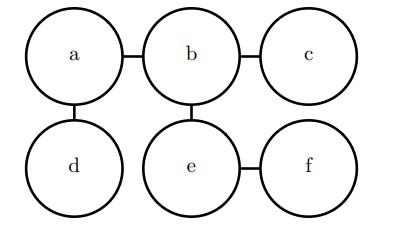
\includegraphics[width=2in]{figure/example/DAG.jpg}
  \caption{}
  \label{fig:2-15}
\end{figure}

\quad \\

接下来正式理解能量模型。如何理解能量模型(EBMs),比如在一个复杂系统里你要表示一个变量的概率$P(x)$,要满足如下性质:
\begin{itemize}
    \item $P(x)> 0$
    \item 所有变量概率之和为1
    \item 方便计算
\end{itemize}

你就可以想到用指数函数(因为大于0)。因此$P(x)$可以表示为$P(x) = e^{f(x)}$,其中$f(x)$ 是关于$x$的函数。

加上归一化因子$Z = \sum_{x \in X}e^{f(x)}$之后,$P(x)$可以表示为:$P(x) = \frac{1}{Z}e^{f(x)}$,其中$\sum_{i=0}^N \frac{e^{f(x_i)}}{\sum_{x \in X} e^{f(x)}} = 1$,满足所有变量概率之和为1,因此$P(x)$ 公式可以用Softmax函数表示:
\begin{align}
&P(x) = \frac{e^{f(x)}}{\sum_{x \in X}e^{f(x)}}
\end{align}

\quad \\

对比上面的概率函数,我们可以通过引入能量函数$E(x)$(能量模型)构建未归一化的概率函数:
\begin{align}
&P(x) = exp(-E(x))
\end{align}

我们可以完全自由地选择那些能够简化学习过程的能量函数。如果我们直接学习各个团势能,我们需要利用约束优化方法来任意地指定一些特定的最小概率值,保证团这个约束条件成立。学习能量函数的过程中,我们可以采用无约束的优化方法。基于能量的模型中的概率可以无限趋近于0,但是永远达不到0。

在统计物理中,服从上式中的任意分布都是玻尔兹曼(吉布斯)分布,正是基于这个原因,我们把许多基于能量的模型称为玻尔兹曼机(Boltzmann Machine) 。通过归一化概率函数,我们可以得到玻尔兹曼分布如下式所示(也就是关于能量函数$E(x)$的复合softmax函数)\footnote{如何用通俗的语言解释「玻尔兹曼分布」?\url{https://www.zhihu.com/question/274174763/answer/662321500}}:
\begin{align}
&P(x) = \frac{e^{-E(x)}}{\sum_{x \in X}e^{-E(x)}}
\end{align}

可以发现,将之前的$f(x)$替换成$-E(x)$,我们就可以建模出一个能量模型了。最简单能量建模方法就是利用$x,y$的Gibbs分布来描述$x,y$之间的能量,即$g_y(x) = -E(x,y)$。这里注意能量模型中$-E(x)$带负号。

通常在机器学习中$E(x)$通常可以表示为似然函数或者对数似然或者值函数,所以有时候求最大似然就可以表示为求最小能量。

比如在分类问题中,对于特征$X = \{x_1,x_2,...,x_n\}$和标签$y \in Y$,我们可以建立能量函数$E(X,y)$,这时候能量函数代表着$X$和$y$的匹配程度,能量越低,$P(x)$越大,匹配程度越好(能量越低匹配越稳定,可以结合高中化学知识进行理解:化学物质能量越低越稳定,键能越大越稳定)。

如图\href{fig:2-15}{2-15}所示,能量函数$E(a,b,c,d,e,f)$可以写为:
\begin{align}
&E(a,b,c,d,e,f) = E_{a,b}(a,b) + E_{b,c}(b,c) + E_{a,d}(a,d) + E_{b,e}(b,e) + E_{e,f}(e,f)
\end{align}
其中,无向图中的因子$\phi$等于对应负能量的指数,即$\phi_{a,b}(a,b) = exp(-E(a,b))$

许多概率图模型算法不需要直接计算$p_{model}(x)$,而只需要计算$log p_{model}(x)$。对于具有因变量$h$的能量模型,可以表示为所有关于$h$的负能量($-E(x,h)$)的指数累加和的形式。有些算法会将该量的负数称为自由能(free energy):
\begin{align}
&F(x) = -log \sum_h exp(-E(x,h))
\end{align}

%\subsubsection{吉布斯分布}

%在物理学中,吉布斯分布又称为玻尔兹曼分布。亥姆霍兹自由能是等温下做所有功的能力,亦称功函
%吉布斯自由能是等温等压下除体积功以外的功的能力
%https://wenku.baidu.com/view/6892c815783e0912a3162a29.html
%自由能是指在某一个热力学过程中,封闭系统减少的内能中可以转化为对外做功的部分,它衡量的是:在一个特定的热力学过程中,系统可对外输出的“有用能量”。可分为亥姆霍兹自由能和吉布斯自由能。
%吉布斯─亥姆霍兹方程,是对计算系统的吉布斯自由能变化的有用热力学公式。为一温度函数。此方程式以约西亚·吉布斯与赫尔曼·冯·亥姆霍兹来命名。
%(https://baike.baidu.com/item/%E5%90%89%E5%B8%83%E6%96%AF-%E4%BA%A5%E5%A7%86%E9%9C%8D%E5%85%B9%E6%96%B9%E7%A8%8B/20109124#1)

%\subsubsection{零样本学习(zero-shot learning)}

%零样本学习(zero-shot learning):\href{https://www.zhihu.com/question/50996014}{https://www.zhihu.com/question/50996014}

\subsubsection{小样本学习(few-shot learning)}

Kang在本文中\cite{kang2019few}提出小样本学习。对于小样本的学习,一般需要分成两步:一是利用base类别的充足样本进行模型的训练,得到的base模型能够提取出base 类的底层特征;二是在base模型的基础上,利用new 类别的小样本对模型进行finetune,得到new模型
\footnote{小样本学习 \quad \url{https://zhuanlan.zhihu.com/p/115246212}{https://zhuanlan.zhihu.com/p/115246212}}。

网络结构如图\href{fig:2-7}{2-7}所示,整体架构分成Feature Extractor、Reweighting Module、Prediction Layer三个部分。
\begin{figure}
  \centering
  % Requires \usepackage{graphicx}
  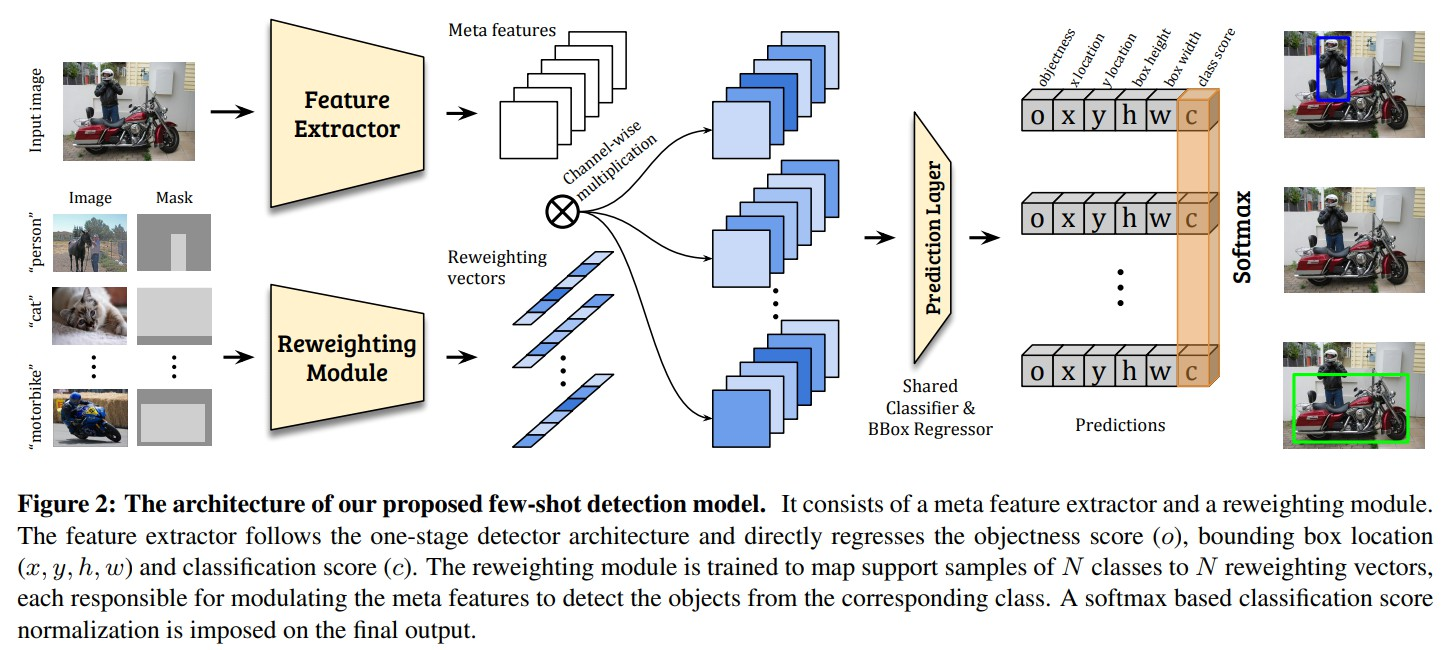
\includegraphics[width=6in]{figure/example/FewShot2.jpg}\\
  \caption{few-shot learning网络结构图}
  \label{fig:2-7}
\end{figure}

\begin{enumerate}
    \item Feature Extractor输入Query images,使用其Backbone (DarkNet)来提取元特征。
    \item 在Reweighting模块中,输入的是Support images、以及images中唯一的1个mask (不管有多少个目标,只选其中一个——“从这个角度看,此文不是完整意义上的目标检测”),为了区分背景和前景,该模块沿着通道方向进行concat($H*W*4$),包括RGB+mask。 借助Support images和Reweighting模块来开始调整Feature Extractor 的元特征。具体而言,将Reweighting模块作为$1 \times 1$的depth-wise卷积核权重,通过卷积元特征进行模型的finetune。
    \item 当有N个新的类别的时候,Reweighting module会产生N个Reweighting vectors, 每一个都负责检测一个新的类别,这些权重向量主要是做分类用的。之后再送入Prediction Layer(head部分)进行分类和回归。
\end{enumerate}

\subsubsection{增量学习}

增量学习主要表现于两个方面:一方面由于其无需保存历史数据,从而减少存储空间的占用;另一方面增量学习在当前的样本训练中充分利用了历史的训练结果,从而显著地减少了后续训练的时间。

增量学习主要有两方面的应用:一是用于数据库非常大的情形,例如Web日志记录;二是用于流数据,因为这些数据随着时间在不断的变化,例如股票交易数据.另外在增量学习中,现有的增量学习算法大多采用决策树和神经网络算法实现的,它们在不同程度上具有以下两方面的缺点:
\begin{enumerate}
    \item 由于缺乏对整个样本集期望风险的控制,算法易于对训练数据产生过量匹配;
    \item 由于缺乏对训练数据有选择的遗忘淘汰机制,在很大程度上影响了分类精度。
\end{enumerate}

最简单的方法之一是增量学习存储的所有数据允许重新训练。在另一个极端是数据的训练、一个实例接一个实例,一个流行的在线学习。采用在线学习算法的方法已经实现增量学习但没有考虑所有的学习问题,特别是学习的新类。



